\documentclass{article}
\usepackage[utf8]{inputenc}
\usepackage{hyperref}
\usepackage[letterpaper, portrait, margin=1in]{geometry}
\usepackage{enumitem}
\usepackage{amsmath}
\usepackage{booktabs}
\usepackage{graphicx}
\usepackage{hyperref}
\usepackage{titlesec}
\usepackage[section]{placeins}

\hypersetup{
colorlinks=true,
    linkcolor=black,
    filecolor=black,      
    urlcolor=blue,
    citecolor=black,
}

  
\title{Economics 7103 - Homework 3}
\author{Ana Mazmishvili}
\date{ February 3, 2024 }
  
\begin{document}
  
\maketitle 
\section{Description of the problem}
Suppose that for a home \(i\), you think the underlying relationship between electricity use and predictor
variables is 
\begin{align} 
     y_i= e^{\alpha} \delta^{d_i} z_i^\gamma e^{\eta_i} 
\end{align}
where 
\begin{itemize}
    \item \(e\) is Euler’s number or the base of the natural logarithm 
    \item \(d_i\) is a binary variable equal to one if home \(i\) received the retrofit program
    \item \(z_i\) is a vector of the other control variables
    \item \(\eta_i\) is unobserved error 
    \item \({\alpha, \delta, \gamma}\) are parameters to estimate.
\end{itemize}

\subsection*{Question 1.a} 
Show that \(ln(y_i)= \alpha + ln(\delta)d_i + \gamma ln(z_i) + \eta_i\)

\textbf{Response:} 
The given equation, \(y_i= e^{\alpha} \delta^{d_i} z_i^\gamma e^{\eta_i}\), represents a power regression model, which is a non-linear regression model. To transform it into a linear regression model, we need to take the natural log of both sides of the equation. We call this log-log transformation. I will use the properties of logarithms and exponential functions in this transformation:
\begin{itemize}
    \item \textbf{Taking log:} \(ln(y_i)= ln(e^{\alpha} \delta^{d_i} z_i^\gamma e^{\eta_i})\)
    \item \textbf{Product Rule:} \(ln(y_i)= ln(e^{\alpha})+ln(\delta^{d_i}) + ln(z_i^\gamma)+ln(e^{\eta_i})\)
    \item \textbf{Power Rule:} \(ln(y_i)= \alpha ln(e)+ln(\delta)d_i + \gamma ln(z_i) +\eta_iln(e)\)
    \item \textbf{The natural logarithm of \(e\) = 1:} \(ln(y_i)= \alpha + ln(\delta)d_i + \gamma ln(z_i) + \eta_i\)      
\end{itemize}





\subsection*{Question 1.b} What is the intuitive interpretation of \(\delta\) ? 

\textbf{Response:} 
If we divide the conditional expectations of the original equation for the treated group by the conditional expectation of the same equation for the untreated group, we will obtain: 
       \begin{align}
       \frac{\E[y_i|d_i=1,z_i]}{\E[y_i|d_i=0,z_i]} = \frac{e^\alpha\delta^1 z_i^{\gamma}e^{\eta_i}}{e^\alpha \delta^0 z_i^{\gamma}e^{\eta_i}} = \frac{e^\alpha\delta z_i^{\gamma}e^{\eta_i}}{e^\alpha z_i^{\gamma}e^{\eta_i}} = \delta
    \end{align}
           
So, as we saw \(\delta\) is the ratio between the expected electricity consumption of the treated and the untreated houses.

\subsection*{Question 1.c} Show that\(\frac{\triangle y_i}{\triangle d_i} = \frac{\delta -1}{\delta^{d_i}} y_i \). What is the intuitive interpretation of \(\frac{\triangle y_i}{\triangle d_i} \).

\textbf{Response:} 

From previous section, we saw that 
\begin{align}
       E[y_i|d_i=1,z_i] = E[y_i|d_i=0,z_i]\delta 
    \end{align}
Since \(d_i\) is a binary variable, \(\frac{\Delta y_i}{\Delta d_i}\) is the difference in the expected value of \(y_i\) between the treatment and control group. So, \[  \frac{\Delta y_i}{\Delta d_i}=\E[y_i|d_i=1,z_i]-\E[y_i|d_i=0,z_i] = \E[y_i|d_i=0,z_i]\delta-\E[y_i|d_i=0,z_i] = (\delta - 1) \E[y_i|d_i=0,z_i] \]
 
To find what \(\E[y_i|d_i=0]\) mean, we can apply the potential outcome framework. Namely, \(y_{0i}\) is the potential outcome of \(y_{i}\) when  \(d_i=0\) and \(y_{1i}\) when \(d_i=1\). According to the potential outcome framework, the log-transformed equation could be rewritten the following way
    \[\ln(y_i)=\ln(y_{0i})+[\ln(y_{1i})-\ln(y_{0i})]d_i \]  

As we saw in previous section, \(y_{1i}/y_{0i}=\delta\).

       \[ \ln (\frac{y_i}{y_{0i}})=d_i\ln(\frac{y_{1i}}{y_{0i}})=d_i\ln(\delta) \]  
        \[ \frac{y_i}{y_{0i}}=e^{d_i\ln(\delta)}=\delta^{d_i} \]  
         \[  y_{0i}=\frac{1}{\delta^{d_i}}y_i \] 
          \[ \frac{\Delta y_i}{\Delta d_i}=(\delta - 1) \E[y_i|d_i=0,z_i]= (\delta - 1) y_{0i} = \frac{\delta-1}{\delta^{d_i}}y_i\]

\(\frac{\Delta y_i}{\Delta d_i}\) shows the change in monthly electricity consumption in kWh if a HH is treated (If a HH received a retrofit).
 
\subsection*{Question 1.d} Show that \(\frac{\partial y_i}{\partial z_i} = \gamma \frac{y_i}{z_i}\). What is the intuitive interpretation of \(\frac{\partial y_i}{\partial z_i}\) when \(z_i\) is the size of the home in square feet?

\textbf{Response:}
\begin{align}
    \frac{\partial y_i}{\partial z_i} = \frac{\partial (e^{\alpha} \delta^{d_i} z_i^\gamma e^{\eta_i})}{\partial z_i} = 
                                       e^{\alpha} \delta^{d_i} \gamma z_i^{\gamma - 1} e^{\eta_i} = 
                                      e^{\alpha} \delta^{d_i} z_i^\gamma e^{\eta_i} \gamma z_i^{- 1} = 
                                      \gamma \frac{y_i}{z_i}
                                      \end{align}
\(\frac{\partial y_i}{\partial z_i}\) describes the marginal change in the electricity consumption of HHs when the size of the home in square feet changes. 

\subsection*{Question 1.e}
\textbf{Response:} 
Estimated parameters and the average marginal effects of \(z_i\) and \(d_i\) are presented in the table \ref{tab:parameters}. The 95\% confidence intervals are displayed in the square brackets. 

\begin{table}[hbt!]
    \centering
    \begin{tabular}{lccc}
\toprule
 & Parameter estimates & AME estimates \\
\midrule
Constant & -0.769000 &   \\
  & [-1.93, 0.315] &   \\
=1 if home received retrofit & 0.904000 & -113.975000 \\
  & [0.894, 0.915] & [-127.401, -99.894] \\
Square feet of home & 0.894000 & 0.629000 \\
  & [0.88, 0.908] & [0.617, 0.64] \\
Outdoor average temperature (\textdegree F) & 0.281000 & 3.997000 \\
  & [0.048, 0.541] & [0.682, 7.759] \\
Observations & 1000 & 1000 \\
\bottomrule
\end{tabular}

    \caption{Estimated parameters and AME (Python)}
    \label{tab:parameters}
        \end{table}

\FloatBarrier
\subsection*{Question 1.f}
\textbf{Response:} 
The Figue \ref{fig:CI} presents the average marginal effects of outdoor temperature and square feet of the home with
bands.

\begin{figure}[hbt!]
    \centering
    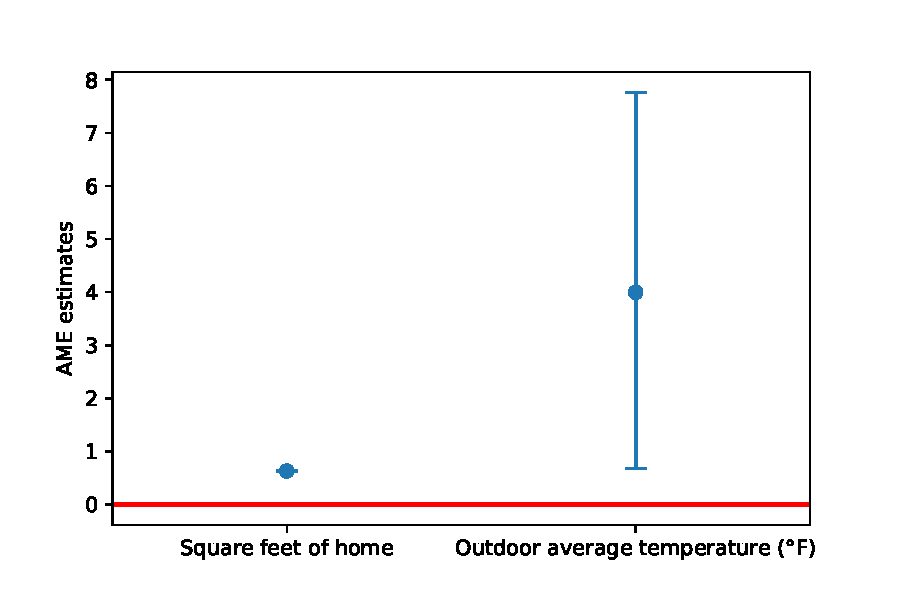
\includegraphics[scale = 0.7]{homework 3/output/figure/hw3ame.pdf}
    \caption{AME of outdoor temperature and square feet of the home with bands for their bootstrapped confidence intervals}
    \label{fig:CI}
\end{figure}



\end{document}